\documentclass[11pt,twoside,a4paper]{article}
%=============== En−Tete ===============
%−−− Insertion de paquetages (optionnel) −−−
%\documentclass[10pt,a4paper]{article}
\usepackage[utf8]{inputenc}
\usepackage[T1]{fontenc}
\usepackage[french]{babel}
\usepackage{fancyhdr}
\usepackage{graphicx}
\usepackage{amssymb}
\usepackage{verbatim}
\usepackage{hyperref}
\usepackage{color}
\usepackage{float}
\hypersetup{ 
dvips, 
backref=true, %permet d'ajouter des liens dans... 
pagebackref=true,%...les bibliographies 
hyperindex=true, %ajoute des liens dans les index. 
colorlinks=true, %colorise les liens 
breaklinks=true, %permet le retour à la ligne dans les liens trop longs 
urlcolor= blue, %couleur des hyperliens 
linkcolor= blue, %couleur des liens internes 
bookmarks=true, %créé des signets pour Acrobat 
bookmarksopen=true}  
\usepackage{geometry}
\geometry{hmargin=2cm,vmargin=3cm}

%−−− Pour le titre −−−
\title{\Huge{RAPPORT DE PROJET}}
\author{{\it Réalisé par :} DIOUBATE SEKOU et SANY ABDOUGUAFAROU, 1ère année LSI}

%=============== Corps ===============
\begin{document}

\maketitle % ´ecrit le titre
\paragraph{}
\begin{figure}[!h]
\begin{center}
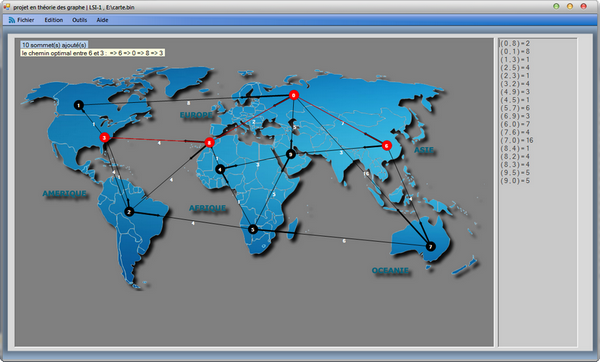
\includegraphics{ecranPrincipal.png}
\caption{La fenêtre principale avec une carte itinéraire}
\end{center}
\end{figure}

\underline{{\it Théorie des graphes}}
\newpage
\tableofcontents % ´ecrit la table des mati`eres

\newpage
\section{Introduction}

Dans ce rapport de projet de théorie des graphes, nous présentons une application desktop que nous avons développée à bases des notions appris en cours.

Pour concrétiser notre projet, nous avons décider de mettre en place un système de d'itinéraire à travers une carte afin de permettre les touristes, voyageurs désirant parcourir plusieurs pays, de mieux optimiser leur chemin. Cette application pourra servir dans plusieurs autres domaine que celui ci.
\paragraph{}
Cette application permet de faire la représentation d'un graphe orienté et non orienté, ainsi que se compose des fonctionnalités et algorithmes suivantes:
\begin{itemize}
	\item Ajouter des Nœuds
	\item  Supprimer des Nœuds
	\item Lier les Nœuds
	\item Générer la Matrice adjacente
	\item Donner Liste adjacent
	\item Modifier le graphe
	\item Enregistrer le graphe
	\item Ouvrir un graphe existant
	\item Faire le parcours en profondeur (algorithme  Depth First Search)
	\item Faire le parcours en largeur (algorithme Breadth First Search)
	\item Faire une fermeture transitive (algorithme de Warshall)
	\item Trouver le chemin le plus cours entre deux Nœud (algorithme Dijkstra)
	\item Générer en détail un rapport général sur le graphe.
 \end{itemize}
\paragraph{}
Dans ce rapport, nous parlerons d’abord de la théorie des graphes en premier lieu , où nous rappellerons l’historique et ce que c’est qu’un graphe, ainsi que quelques définitions de base de cette matière ;

 Ensuite, on présentera les fonctionnalités de notre application ainsi qu’une explication détaillée sur l'implémentation du programme. Puis une conclure.

\newpage
\section{La théorie des graphes }

\subsection{Historique de la théorie des graphes}

La théorie des graphes est très probablement née en 1735 lorsque Leonhard Euler (1707 - 1783) résout le problème des sept ponts de Königsberg (De nos jours Kaliningrad en Russie). Ce problème est très simple sur le principe mais un peu plus compliqué à démontrer, en voici l'énoncé : La vile de Königsberg est une ville autour d'un fleuve, elle compte quatre berges et sept ponts les reliant. Le but du jeu est de savoir s'il existe un chemin permettant d'emprunter tous les ponts une fois et une seule et revenir au point de départ. Le problème s'appelle, de façon plus formelle, la recherche d'un cycle eulérien dans un graphe. Euler a démontré que ce problème n'avait pas de solution.


\subsection{Définition du graphe}


En informatique, un graphe c'est une structure de donnée tout comme les tableaux, composée de nœuds interconnecter entre eux par des liens. Chaque nœud contient une ou plusieurs données de n’importe quel type.
Un graphe est composé de sommets et d'arcs  pour les graphes non orientés ou d'arêtes pour les graphes orientés. Un graphe G est défini de manière formelle par un couple (S, A) où :
\begin{itemize}
	\item {\bf S} est un ensemble fini d'éléments. Chacun de ces éléments est appelé sommet du graphe.
	\item {\bf A} est un sous ensemble (éventuellement nul) de SxS. Chacun de ces éléments de A est appelé arc ou arête. L'ensemble A est donc composé de paires ( x , y ) où x et y étant appelés les extrémités de l'arc du graphe non orienté et appelés respectivement le départ et l’arrivé de l'arête pour les graphes orienté.
\end{itemize}


\newpage 
\section{Présentation de application}

\begin{figure}[!h]
\begin{center}
\caption{La fenêtre principale: carte itinéraire}
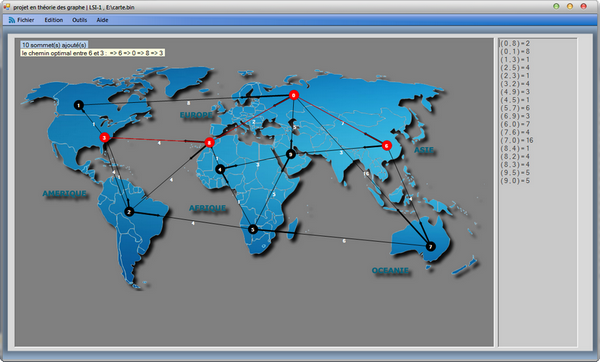
\includegraphics{ecranPrincipal.png}
\caption{La fenêtre principale}
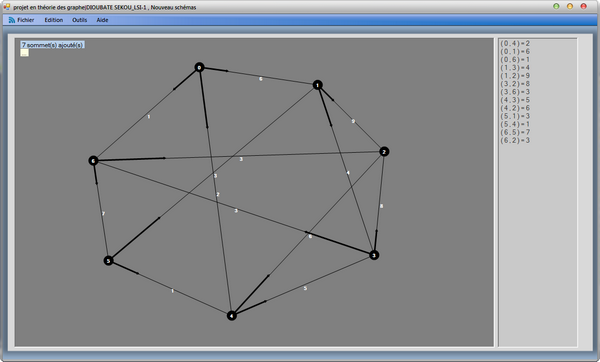
\includegraphics{ecranPrincipal2.png}
\end{center}
\end{figure}
\newpage

\section{Fonctionnalités d’application}

\subsection{Représentation du graphe}
Comme nous l’avons introduit plus haut, cette application permet de faire la représentation d'un graphe orienté et non orienté à travers les fonctions d’ajout et suppression des Nœuds ainsi que la fonction de liaison pour faire, suivant l’orientabilité du graphe, un arc ou une arête entre les Nœuds.
\begin{figure}[!h]
\begin{center}

\includegraphics{menu.png}
\caption{Menu principal}
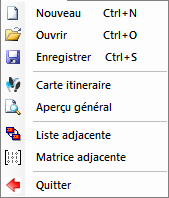
\includegraphics{fichier.png}
\caption{Menu Fichier}
\end{center}
\end{figure}
{\bf Pour faire un nouveau graphe, on procède comme suit :} 
\begin{itemize}
  	 \item \textbf{Fichier => Nouveau} \textit{ (raccourci clavier : control + N)};
	\item \textbf{Selectionner} le type de graphe(graphe orienté ou graphe non orienté) dans la boite de dialogue apparaissant;
	\item \textbf{Cocher} si avec ou sans carte dans la même boite de dialogue apparaissant;
\begin{figure}[!h]
\begin{center}
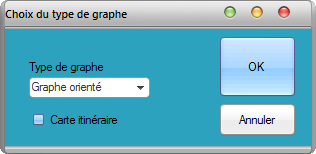
\includegraphics{choix.png}
\caption{Choix du type de graphe}
\end{center}
\end{figure}
	\item puis \textbf{OK} pour commencer;
\end{itemize}
Le curseurs vous donne la main pour  placer les Noeuds:
\begin{itemize}
	\item \textbf{Click gauche} dans l’espace de traçasse pour placer des nœuds (autant de nœuds souhaités);
	\item \textbf{Click droite} pour finir, et le curseur redevient à son état initial, une flèche.
\end{itemize}
\subsection{Modification}
Une fois le graphe élaboré et tracé, on pourra le modifier par les fonctions d’ajouter, de suppression et de liaison, mais aussi déplacer ces nœuds et les ajuster.
\begin{figure}[!h]
\begin{center}

\includegraphics{menu.png}
\caption{Menu principal}
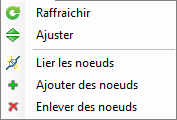
\includegraphics{edition.png}
\caption{Menu  edition}
\end{center}
\end{figure}

{\bf Pour  ajouter des nœuds:}
\begin{itemize}
	\item \textbf{Edition => Ajouter des nœuds}; 
	\item \textbf{Click gauche} dans l’espace de tracasse pour placer des nœuds (autant de nœuds souhaités);
	\item \textbf{Click droite} pour finir.
\end{itemize}
\paragraph{}
{\bf Pour supprimer des nœuds:}
\begin{itemize}
	\item \textbf{Edition => Enlever les Nœuds};
	\item \textbf{Cocher} le numéro des nœuds à supprimer, puis OK.
\begin{figure}[!h]
\begin{center}
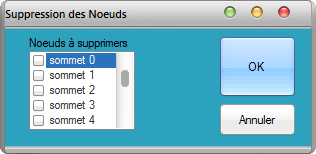
\includegraphics{supprimer.png}
\caption{Supression des Noeuds}
\end{center}
\end{figure}
\end{itemize}
\paragraph{}
{\bf Pour faire des liaisons :}
\begin{itemize}
	\item \textbf{Edition => lier les Nœuds};
	\item \textbf{Cliquer} dans un nœud de départ puis dans un nœud d’arrivé.
	\item \textbf{Taper} ensuite le cout de la liaison dans la boite de dialogue apparaissant. Avec la possibilité de faire autant de liaisons souhaitées; 
	\item \textbf{Cliquer} sur le bouton terminer pour finir.
\end{itemize}
\paragraph{}
{\bf Pour déplacer un nœud:}
\begin{itemize}
	\item \textbf{Cliquer} sur le nœud à déplacer puis sur le nouvel emplacement souhaiter dans l’espace de traçasse.
\end{itemize}

\subsection{Modification avec la matrice d’adjacence}
On a également la possibilité d’utiliser \textbf{la matrice d’adjacence} pour faire des modifications dans la structure du graphe. Pour se faire, il suffit de changer les valeurs et les champs des couts de la liaison dans la matrice.
\paragraph{}
\begin{figure}[!h]
\begin{center}
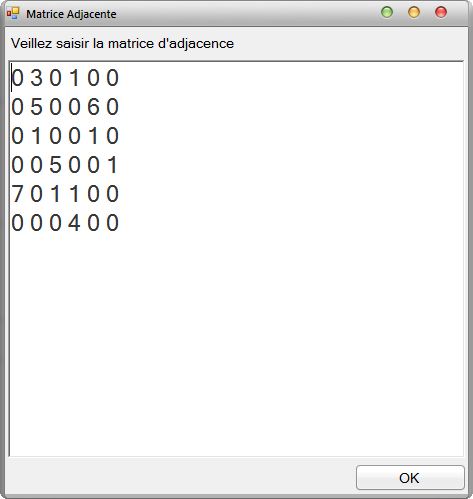
\includegraphics{matrice.png}
\caption{La matrice adjacence}
\end{center}
\end{figure}

\subsection{Sauvegarde et ouverture d’un graphe existant}
Par un sérialisation de type binaire, on pourra enregistrer le graphe ainsi qu'avec tous ses variables, y compris sa matrice d’adjacence, dans un fichier sous format \textit{.bin}. Ce travail pour être ouvert lors d’une exécution ultérieure par une procédure inverse qui est la desérialisation.
\paragraph{}

{\bf On procède ainsi:}
\begin{itemize}
\item \textbf{Fichier => Ouvrir} \textit{ (raccourci clavier : control + O)}
\item \textbf{Fichier => Enregistrer} \textit{  (raccourci clavier : control + S)}
 \end{itemize}

\subsection{Les fonctions d’outils :}
Elles constituent l'exécution des différents algorithme du cours.

\begin{figure}[!h]
\begin{center}

\includegraphics{menu.png}
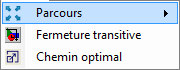
\includegraphics{outil.png}
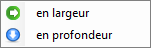
\includegraphics{parcours.png}
\caption{Menu Outil}
\end{center}
\end{figure}
\paragraph{}

{\bf Pour en exécuter une :}
\begin{itemize}
\item \textbf{Outil => parcours}, puis choisir le Nœud de départ.
\item \textbf{Outil => fermeture transitive}
\item \textbf{Outil => chemin optimal}, choisir le nœud de départ et d’arrivé.
 \end{itemize}



\subsection{Autres fonctionnalités}
Avant de boucler cette partie, nous tenons à signaler d’autres fonctions , à savoir :
\begin{itemize}
\item \underline{Le menu contextuel}:
	En plus des raccourcis clavier, l'application possède un menu contextuel qui permet d'accéder plus facilement aux différents fonctionnalités du programme.
	\begin{figure}[!h]
	\begin{center}
	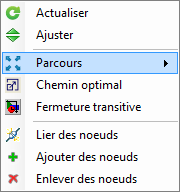
\includegraphics{contextuleMenu.png}	
	\caption{Le menu contextuel}
	\end{center}
	\end{figure}
\item \underline{La barre latéral des arrête }: Elle s'interprète ainsi { \it(noeud A , noeud B) = cout de A à B}
\item \underline{La liste d’adjacence}:
	Elle permet de visionner pour un noeud donné, toutes les liaisons entrantes et sortant de ce noeud.
\item \underline{Rapport}:
	Elle donne tous les renseignement sur le graphe, à savoir:  la taille du graphe, la matrice, la liste et les résultats des  différents algorithmes  appliqués au graphe.



 \end{itemize}
\newpage

\section{L’implémentation du programme}

Pour implémenté de cette application on a eu recours à l’utilisation du langage de programmation C-Sharp. Ce choix se rapport non seulement par sa simplicité et sa puissance mais surtout par ce que nous la maitrisons mieux que les autres langages de programmation orienté objet (POO).

Le programme est décomposé en deux parties. La première appelée {\bf « forms des graphes »} est , comme son nom l’indique, constituée de {\it WindowsForm}. Et la seconde appelée  {\bf « traitement des graphes »}, est une {\it bibliothèque de classes}.
Commençons par la première qui est la plus importante.


\subsection{Forms des graphes}

C’est l’interface de l’application. Elle contient toutes les fonctions nécessaires au traçage et mise en forme de la représentation du graphe. On y retrouve entre autre :

-les fonctions d’ajout de Nœuds et de liaisons;

-les fonctions de rafraichissement et d’ajustement de la représentation du schéma;

-une classe nommée « classeDuDessin » qui implémente les fonctions qui permettent de dessiner des sommets et des liaisons sur l’interface Windows form;


\subsection{Traitement des graphes}

Cette bibliothèque est le cœur du projet. Elle regroupe  en son sein les classes de structure pour le graphe, telles que :{\it la classe sommet, la classe liaison, la classe graphe et la classe grapheBO}. Ainsi que les classes de l’implémentation des algorithmes de cours qui seront appliqués au graphe, à savoir :{\it la classe parcours, la classe Warsall et la classe Djikstra}.

\subsubsection{La classe « sommet »}
Elle contient les informations sur le Nœud et  principalement : son numéro, ses coordonnées x et y dans le plans, un booléen pour le marquer dans les itérations et deux listes de liaisons entrant et sortant.
\begin{verbatim}
public class sommet
        {
            private int _numero;
            private int _x, _y;
           
            private bool _marquer = false;

            private List<liaison> _Liaisons_sortants;

            private List<liaison> _Liaisons_entrants;

            private int _cout; 
                            // ne pas confondre avec le cout de la liaison
                     //ce cout ne sera utilisé que dans l algo de Djikstra, 

            public sommet precedant;
                       //ce variable aussi est  pour  l algo de Djikstra
        }
\end{verbatim}

\subsubsection{La classe « liaison »}
Elle contient deux variables: le cout de la liaison et le sommet lié.
\begin{verbatim}
 public class liaison
    {
        public int cout;	// le veritable cout de la liaison
        private sommet _sommet_lier;
        public liaison()
        {
            _sommet_lier = null; cout = -1;
        }
        public liaison(ref sommet _sommet_suivant1, int _cout)
        {
            _sommet_lier = _sommet_suivant1; cout = _cout;
        }
    }
\end{verbatim}

\subsubsection{La classe « graphe »}
Elle est principalement la structure du graphe. Elle comporte non seulement la taille du graphe ou le nombre de Nœuds du graphe, mais aussi un tableau de sommet unidimensionnel qui contient l’ensemble des Nœuds. En plus, un tableau d’entiers double dimension qui constitue la matrice d’adjacence des couts. Elle comporte également un booléen indiquant si le graphe est orienté ou non.
\begin{verbatim}
 public class Graphe
    {
        private bool _graphe_orienter;	

        private int _Nombre_de_noeud;

        private sommet[] _table_de_sommets
        public  sommet[] Table_de_sommets
        {
            get { return _table_de_sommets; }
            set { _table_de_sommets = value; }
        }

        int[][] _matrice;//matrice d'adjacence
        public int[][] Matrice
        {
            get { return _matrice; }
            set { _matrice = value; }
        }

        public Graphe()
        {
 
        }
    }
\end{verbatim}

\subsubsection{La classe « grapheBO »}
 Qui pourrait se traduire {\it « graphe Business Objet »}, est la classe dans laquelle on crée un objet de type {\it graphe} et qui contient aussi quelques fonctions appliquées au graphe, telle que : la suppression des nœuds,  la sérialisation et desérialisation.
\begin{verbatim}
  public class GrapheBO
    {
        public static Graphe graphe = new Graphe();	//creation de l objet graphe

        public static void supprimer(int numero)
        {
            int indice_A_supprimer = -1;

            for (int i = 0; i < graphe.Nombre_de_noeud; i++)
            {
                foreach (liaison p in graphe.Table_de_sommets[i].Liaisons_sortants)
                    if (p.Sommet_lier.Numero == numero)
                    {
                        graphe.Table_de_sommets[i].Liaisons_entrants.Remove(p); break;
                    }

                foreach (liaison q in graphe.Table_de_sommets[i].Liaisons_sortants)
                    if (q.Sommet_lier.Numero == numero)
                    {
                        graphe.Table_de_sommets[i].Liaisons_sortants.Remove(q); break;
                    }

                if (graphe.Table_de_sommets[i].Numero == numero)
                {
                    indice_A_supprimer = i;
                    graphe.Table_de_sommets[i].Liaisons_sortants.Clear();
                    graphe.Table_de_sommets[i].Liaisons_entrants.Clear();
                }
            }
            graphe.Nombre_de_noeud --;
            for (int i = indice_A_supprimer; i < graphe.Nombre_de_noeud; i++)
            {
                graphe.Table_de_sommets[i] = graphe.Table_de_sommets[i + 1];
                graphe.Matrice[i] = graphe.Matrice[i + 1];
            }

            for (int i = 0; i < graphe.Nombre_de_noeud; i++)
            {
                for (int j = indice_A_supprimer; j < graphe.Nombre_de_noeud; j++)
                {
                    graphe.Matrice[i][j] = graphe.Matrice[i][j + 1];
                }
            }
        }

        public static void serialiser(string filename)
        {
            Stream stream = File.Open(filename, FileMode.Create);
            BinaryFormatter bFormatter = new BinaryFormatter();
            bFormatter.Serialize(stream, graphe);
            stream.Close();
        }

        public static void deserialiser(string filename)
        {
            Graphe mygraf;
            Stream stream = File.Open(filename, FileMode.Open);
            BinaryFormatter bFormatter = new BinaryFormatter();
            mygraf = (Graphe)bFormatter.Deserialize(stream);
            stream.Close();
            graphe.Graphe_orienter = mygraf.Graphe_orienter;
            graphe.Nombre_de_noeud = mygraf.Nombre_de_noeud;
            graphe.Table_de_sommets = mygraf.Table_de_sommets;
            graphe.Matrice = mygraf.Matrice;
        }
    }
\end{verbatim}

\subsubsection{La classe « Warsall » }
Qui, comme son nom l’indique, contient l’implémentation de l’algorithme de WARHALL pour la fermeture transitive.
\begin{verbatim}
 public class Warshall
    {
       public static bool[][] fermeture_transitive() 
       {
           int k, i, j, n=GrapheBO.graphe.Nombre_de_noeud;
           bool[][] matrice_temporaire = new bool[n][];

           for (i = 0; i < n; i++)
           {
               matrice_temporaire[i] = new bool[n];
               for (j = 0; j < n; j++)
                 matrice_temporaire[i][j] = (GrapheBO.graphe.Matrice[i][j] > 0)
                                                                   ? true : false;
           }
           for (k = 0; k < n; k++)
               for (i = 0; i < n; i++)
                   for (j = 0; j < n; j++)
                       matrice_temporaire[i][j] = matrice_temporaire[i][j] 
                       || (matrice_temporaire[i][k] && matrice_temporaire[k][j]);
           return matrice_temporaire;
       }
}
\end{verbatim}

\subsubsection{La classe « Djikstra »}
 Comme son nom l'indique également, implémente le fameux algorithme de DJIKSTRA pour touver le chemin le plus court entre deux noeuds.
\begin{verbatim}
public class Dijkstra
    {
        static List<sommet> les_stations=new List<sommet>();
      
        //On déclare d abord une fonction d ouverture du Sommet de cout minimum
         // parmis les Sommets non visites

        public static sommet ouvre_min(List<sommet> liste)
        {
            sommet res = new sommet();
            res.Cout=int.MaxValue;
            foreach (sommet s in liste)
                {
                    if (s.Cout <= res.Cout)
                        res = s;
                }
            liste.Remove(res);
            return res;
        }

        //l'algo de Dijkstra proprement dit

        public static List<sommet> plus_court_chemin(sommet depart, sommet destination)
        {
	 
           for (int i = 0; i < GrapheBO.graphe.Nombre_de_noeud; i++)    
            {
                les_stations.Add( GrapheBO.graphe.Table_de_sommets[i]);
            }

            List<sommet> chemin = new List<sommet>();
            List<sommet> Sommets_a_ouvrir = new List<sommet>();
            sommet Sommet_ouvert = new sommet(); 

            //on initialise les couts à l'infini pour tous les Sommets 
            foreach (sommet sta in les_stations)
                {
                    sta.Cout=int.MaxValue;
                    sta.precedant=null;
                    Sommets_a_ouvrir.Add(sta);
                }

            depart.Cout=0;
            Sommet_ouvert = ouvre_min(Sommets_a_ouvrir);

            //on verifie qu'il existe au moins un arc liant le Sommet ouvert
           // aux Sommets restants et que l'on n'est pas à l'arrivee
            
            while (Sommet_ouvert != destination)
            {
                foreach (sommet s in Sommets_a_ouvrir)
                    {
                        int val=int.MaxValue;    

                        foreach (liaison l1 in Sommet_ouvert.Liaisons_sortants)
                                if (l1.Sommet_lier.Numero == s.Numero)
                                   val = Sommet_ouvert.Cout +l1.cout;
                       
                        if (s.Cout > val)
                            {
                                 s.Cout=val;
                                 s.precedant=Sommet_ouvert;
                        }
                    }
                    Sommet_ouvert = ouvre_min(Sommets_a_ouvrir);

            }

            Sommets_a_ouvrir.Clear();

            if (destination.Cout == int.MaxValue)
            {
                //le graphe n'est pas connexe, il n y a pas de chemin
                 return null;
            }
            else          
            {
               //construction du chemin 
                while (Sommet_ouvert != depart)
                {
                    chemin.Add(Sommet_ouvert);
                    Sommet_ouvert = Sommet_ouvert.precedant;
                }
            }

            chemin.Add(depart);

            chemin.Reverse();

            return chemin;
        }
    }
\end{verbatim}

\newpage
\section{Conclusion}
Ce projet a été pour nous une grande opportunité d'approfondir nos connaissance dans cette matière qui est la théorie des graphes. En programmant ces algorithmes, nous les avons parfaitement assimiler si l'on peut dise ainsi. Également, ce projet nous a permit  d'apprendre plus sur ce langage de programmation C sharp.



























\end{document}